\documentclass[runningheads]{llncs}
%
\usepackage[T1]{fontenc}
\usepackage{todonotes}
\usepackage{authblk}
\usepackage{graphicx}
\usepackage{amsmath}
\usepackage{caption}
\usepackage{soul}
\usepackage{hyphenat}
\usepackage{pifont}
\usepackage[table]{xcolor}

\newcommand{\tickm}{\ding{52}}
\newcommand{\cross}{\ding{56}}
% Highlight for the baseline condition (Monty default: HSV only, no LTP)
\newcommand{\baserow}{\rowcolor{black!10}}

\begin{document}
%
\title{Texture Feature Enhanced Sensory Module for Improved Object Recognition in a Neocortex-inspired Embodied Sensorimotor Agent (Monty) }
\titlerunning{Texture Feature Enhanced Sensory Module for Monty}

% \author{First Author\inst{1}\orcidID{0000-1111-2222-3333} \and
% Second Author\inst{2,3}\orcidID{1111-2222-3333-4444} \and
% Third Author\inst{3}\orcidID{2222--3333-4444-5555}}
% %
% \authorrunning{F. Author et al.}
% % First names are abbreviated in the running head.
% % If there are more than two authors, 'et al.' is used.
% %
% \institute{Princeton University, Princeton NJ 08544, USA \and
% Springer Heidelberg, Tiergartenstr. 17, 69121 Heidelberg, Germany
% \email{lncs@springer.com}\\
% \url{http://www.springer.com/gp/computer-science/lncs} \and
% ABC Institute, Rupert-Karls-University Heidelberg, Heidelberg, Germany\\
% \email{\{abc,lncs\}@uni-heidelberg.de}}

\author{Pulin Agrawal\inst{1}\orcidID{0000-0003-1477-9863} \and Tristan C Weldon\inst{1} \and Rocco A Leporace\inst{1}}
\authorrunning{P. Agrawal et al.}
\institute{The Pennsylvania State University, The Behrend College, Erie, PA, USA 
\\\email{\{pagrawal, tcw5157, ral5755\}@psu.edu}
}

\maketitle          

\begin{abstract}
Deep learning systems remain data-bound, vulnerable to catastrophic forgetting, and largely disembodied. Monty, the reference implementation of the Thousand Brains Project, offers an alternative. It is a sensorimotor agent that builds object-centric reference frames. It learns an object by moving a sensor across its surface and storing features at pose in a graph, which lets it acquire new objects from a few presentations without the need for retraining. Its sensor module currently extracts morphological features along with a simple hue descriptor, so it cannot separate objects that share a shape but differ in surface texture. We add a texture feature based on the split (Completed) Local Ternary Pattern (LTP). A normalized LTP histogram is computed over each sensed patch and passed to the learning module as a CMP-compliant non-morphological feature. This descriptor requires no pre-training. We compare three LTP encoding schemes, 'ror', 'uniform' and 'multiscale'. We also describe a histogram matching procedure that fixes the distance metric and sets the feature tolerance by maximizing the separation between within-object and across-object patch distances. Bhattacharyya (Hellinger) distance gave the best separation. On the YCB dataset and on a custom YCB-11R dataset, LTP raises recognition accuracy and reduces the number of steps needed to converge on an object in both the ambient and the directional lighting setups.

\keywords{Object Recognition \and Monty \and Thousand Brains Project \and Local Ternary Pattern \and Biologically-inspired }
\end{abstract}




\section{Introduction}

Despite deep learning’s massive success in natural language and computer vision, there are still aspects of human cognitive capacities that these systems lack. Deep learning systems are still training data bound. They need a massive amount of training data repeated over multiple epochs before the model is learned. Learning something new after the training has ended is still a challenge. To prevent catastrophic forgetting \cite{vandeven2025109ContinualLearning,chen2018ContinualLearningCatastrophica} when training the model on a new concept, we need to retrain the model on the entire training data with multiple instances of the new concept before the model can learn it. In addition, typical deep learning has often ignored the importance of embodied learning \cite{paolo2024position,kugele2023embodied,kadambi2026EmbodimentMultimodalLarge,rolla2026EmbodimentChallengeArtificial}. An important aspect of embodiment is sensorimotor learning, where the entity doing the learning has sensors and actuators embedded in the environment and the learning occurs through the process of moving the sensors in the environment and building a model of the environment, much like how human brains do it. To match human cognitive capacity for seeing a new object and rapidly learning to recognize it via sensorimotor learning, we may look for inspiration in the brain. 
 
Monty \cite{2026ThousandbrainsprojectTbpmonty} is such a framework built on the theoretical neuroscience work \cite{thousandbrainsproject2024} done at Thousand Brains Project based on the book by Jeff Hawkins \cite{hawkins2021thousand}. Concepts used by Monty are derived from experimental evidence on how brains work. They do not target biological replication but a biological inspiration. One of their primary long-term goals is to develop a "Cortical Messaging Protocol" (CMP) that can be used as a universal language for communication and building consensus between the proposed "thousand brains", a loosely analogous concept based on a cortical column. Monty is a sensorimotor learning system that uses an active learning mechanism to explore its environment and learn location relevant features on an object to recognize it. Embodiment is therefore a first-class citizen in the foundational principles of this model. Monty stores the features of an object it learned in a graph, which is like the reference frame of the object in the thousand brain's theory, presented in Hawkins' book. Separate reference frames (graphs) allow Monty to rapidly recognize and discriminate new objects within a few iterations of presentation of the object \cite{leadholm2026thousand}. Unlike deep learning systems, it does not undergo catastrophic forgetting and can retain new objects learned for the lifetime of the agent. Although Monty has been shown to be capable of rapidly recognizing distinct objects, currently it does not have the appropriate sensory and feature extraction apparatus to distinguish between objects with different surface texture features. To distinguish between objects that have the same morphology but different textures, we need to be able to sense and attribute other physical features of an object, like color. 
 
Crucially, integrating a new texture feature detector into Monty is a computer vision engineering problem in service of a larger goal of exploring the capabilities of a biologically-inspired cognitive architecture like Monty. Thousand brains theory associates various local sensory features at specific reference frames to build complete object models within individual cortical columns. A non-morphological texture feature sits directly within the Cortical Messaging Protocol used to gather local sensory evidence at a specific surface location. Moreover, the mechanics of our chosen texture descriptor find their biological-inspiration in local contrast-based computations in the visual pathway producing the center-surround receptive field characteristics. 

In this paper we propose a new feature that can be learned for an object by Monty, inspired by the Local Binary Pattern algorithm \cite{ojala2000gray}. This can help Monty distinguish between objects that have the same shape but different surface textures. We use a split variant \cite{rassem2014completed} of Local Ternary Pattern (LTP) \cite{tan2007enhanced} to extract texture features for Monty. Our primary contribution in this paper is a new sensor-module feature for Monty with a split LTP histogram extracted per patch that is CMP-compliant. We compare the performance of various encoding schemes of LTP with our dataset. We also devise a split LTP histogram matching system that helps us identify the distance metric and tolerance parameters to effectively discriminate objects with similar shape under the Monty evidence matching protocol. 
Crucially, integrating a new texture feature detector into Monty is a computer vision engineering problem in service of a larger goal of exploring the capabilities of a biologically-inspired cognitive architecture like Monty. Thousand brains theory associates various local sensory features at specific reference frames to build complete object models within individual cortical columns. A non-morphological texture feature sits directly within the Cortical Messaging Protocol used to gather local sensory evidence at a specific surface location. Moreover, the mechanics of our chosen texture descriptor find their biological-inspiration in local contrast-based computations in the visual pathway producing the center-surround receptive field characteristics.  We demonstrate the effectiveness of this method by showing increased accuracy and efficiency with the standard YCB dataset and a custom dataset `YCB-11R'. 

\section{Background}
\subsection{Thousand Brains Theory}

The Thousand Brains Theory is a neuro-science inspired framework, developed by Jeff Hawkins and colleagues at Numenta, that proposes a unified account of how the neocortex gives rise to intelligence \cite{hawkins_framework_2019,hawkins2021thousand}. This work is built on Mountcastle's \cite{mountcastle_columnar_1997} hypothesis that a cortical column is a single repeating circuit that underlies all cortical computation. A central claim of the theory is that grid-cell-like mechanisms exist throughout the neocortex in every region and column. Cortical columns in the sensory regions establish object-centric reference frames in which sensory input is represented \cite{hawkins_framework_2019}. Because columns receive input from different sensors and locations, they learn models of objects through movement of the sensors, much as grid and place cells learn models of environments through movement of the body in the hippocampus \cite{hafting2005MicrostructureSpatialMap}. The resulting redundancy of evidence about a sensory object is a feature of the system that helps reconcile uncertain inputs through a consensus or "voting" process. The theory holds that each cortical column in the brain generates its own sensory-motor model of the world using these mechanisms, acting as a mini-brain. The theory advances this as the basis for robust perception, compositional knowledge, and continual sensorimotor learning \cite{hawkins2017theory,hawkins_framework_2019}. 

\subsection{Monty}

Monty is the first practical implementation of a "thousand-brains system", developed by the Thousand Brains Project, an open-source research initiative launched by Numenta in 2024. The Thousand Brains Project is currently an independent non-profit entity developing brain-based alternatives to deep learning \cite{thousandbrainsproject2024}. Monty is a sensorimotor agent intended to embody the operating principles of the neocortex and, eventually, to implement any capability the cortex supports. In contrast to mainstream deep-learning systems that ingest static datasets through a single model over many training epochs, Monty is a sensorimotor system that learns by actively interacting with and sensing different parts of the world over time. It has many sensory and learning units structuring its knowledge through reference frames \cite{thousandbrainsproject2024}. Monty uses cortical columns in the neocortex \cite{mountcastle_columnar_1997} as a loose inspiration for its modules. According to the thousand brains theory, these modules interact with each other to build a consensus of what is currently being sensed. Monty uses "Cortical Messaging Protocol" (CMP) to communicate these messages across the modules. Recent empirical work evaluating Monty on 3D object recognition and pose estimation with the YCB object dataset reports that its structured, sensorimotor-derived representations support robust generalization, sensitivity to global shape and object symmetry, and accelerated inference through a modular voting algorithm \cite{leadholm2021grid,leadholm2026thousand}. 
 
\subsubsection{Sensory Module}
Monty’s sensor module \cite{2026ThousandbrainsprojectTbpmonty} consists of a collection of stimuli feature extractors which are modality specific. The extracted features are tagged with the current positional and rotational information of the sensor, called ‘pose’. Further, the extracted features are also categorized as morphological (like curvature, position, etc.) and non-morphological (like color, texture, etc.) features. Collectively, a sensor module output can be thought of as `features at pose'. 

\subsubsection{Learning Module}
The learning module in Monty \cite{2026ThousandbrainsprojectTbpmonty} may use one of many possible algorithms for recognizing an object. The current implementation uses EvidenceGraphLM. This type of learning module uses locations stored in a graph model maintained for each uniquely identifiable object. During an episode of learning, features at various locations are recorded and stored in this graph. During inference, from the set of all possible identifiable objects, a hypothesis table is built, which accumulates evidence as the sensor moves and records stimuli feature observations. The learning module matches the `features at pose' with objects in the hypothesis table, consisting of possible graphs given those features and sensor displacements. Each feature is matched to the targets’ feature at that displacement. A distance metric (\textit{d}) is computed between the target feature and the features at the current pose. The evidence contribution of the feature is measured, with the tolerance hyperparameter, as: $$max(0, 1-\textit{d}/tolerance)$$ 
When \textit{d}>tolerance the feature contribution is 0. Otherwise, as \textit{d} approaches 0, more and more evidence, weighted by the feature’s weight, is added to the total accumulated evidence for the target hypothesis. Feature weights are normalized before they get applied so that no more than a unit of total evidence is added per step across all the features combined. The object with the most accumulated evidence is the most likely hypothesis of the object under observation. Based on a threshold, hypotheses are pruned from the table until only one is left, or the maximum number of steps is reached.  

\subsection{From Local Binary to Ternary Patterns}

\begin{figure}
\vspace{-10pt}
\centering
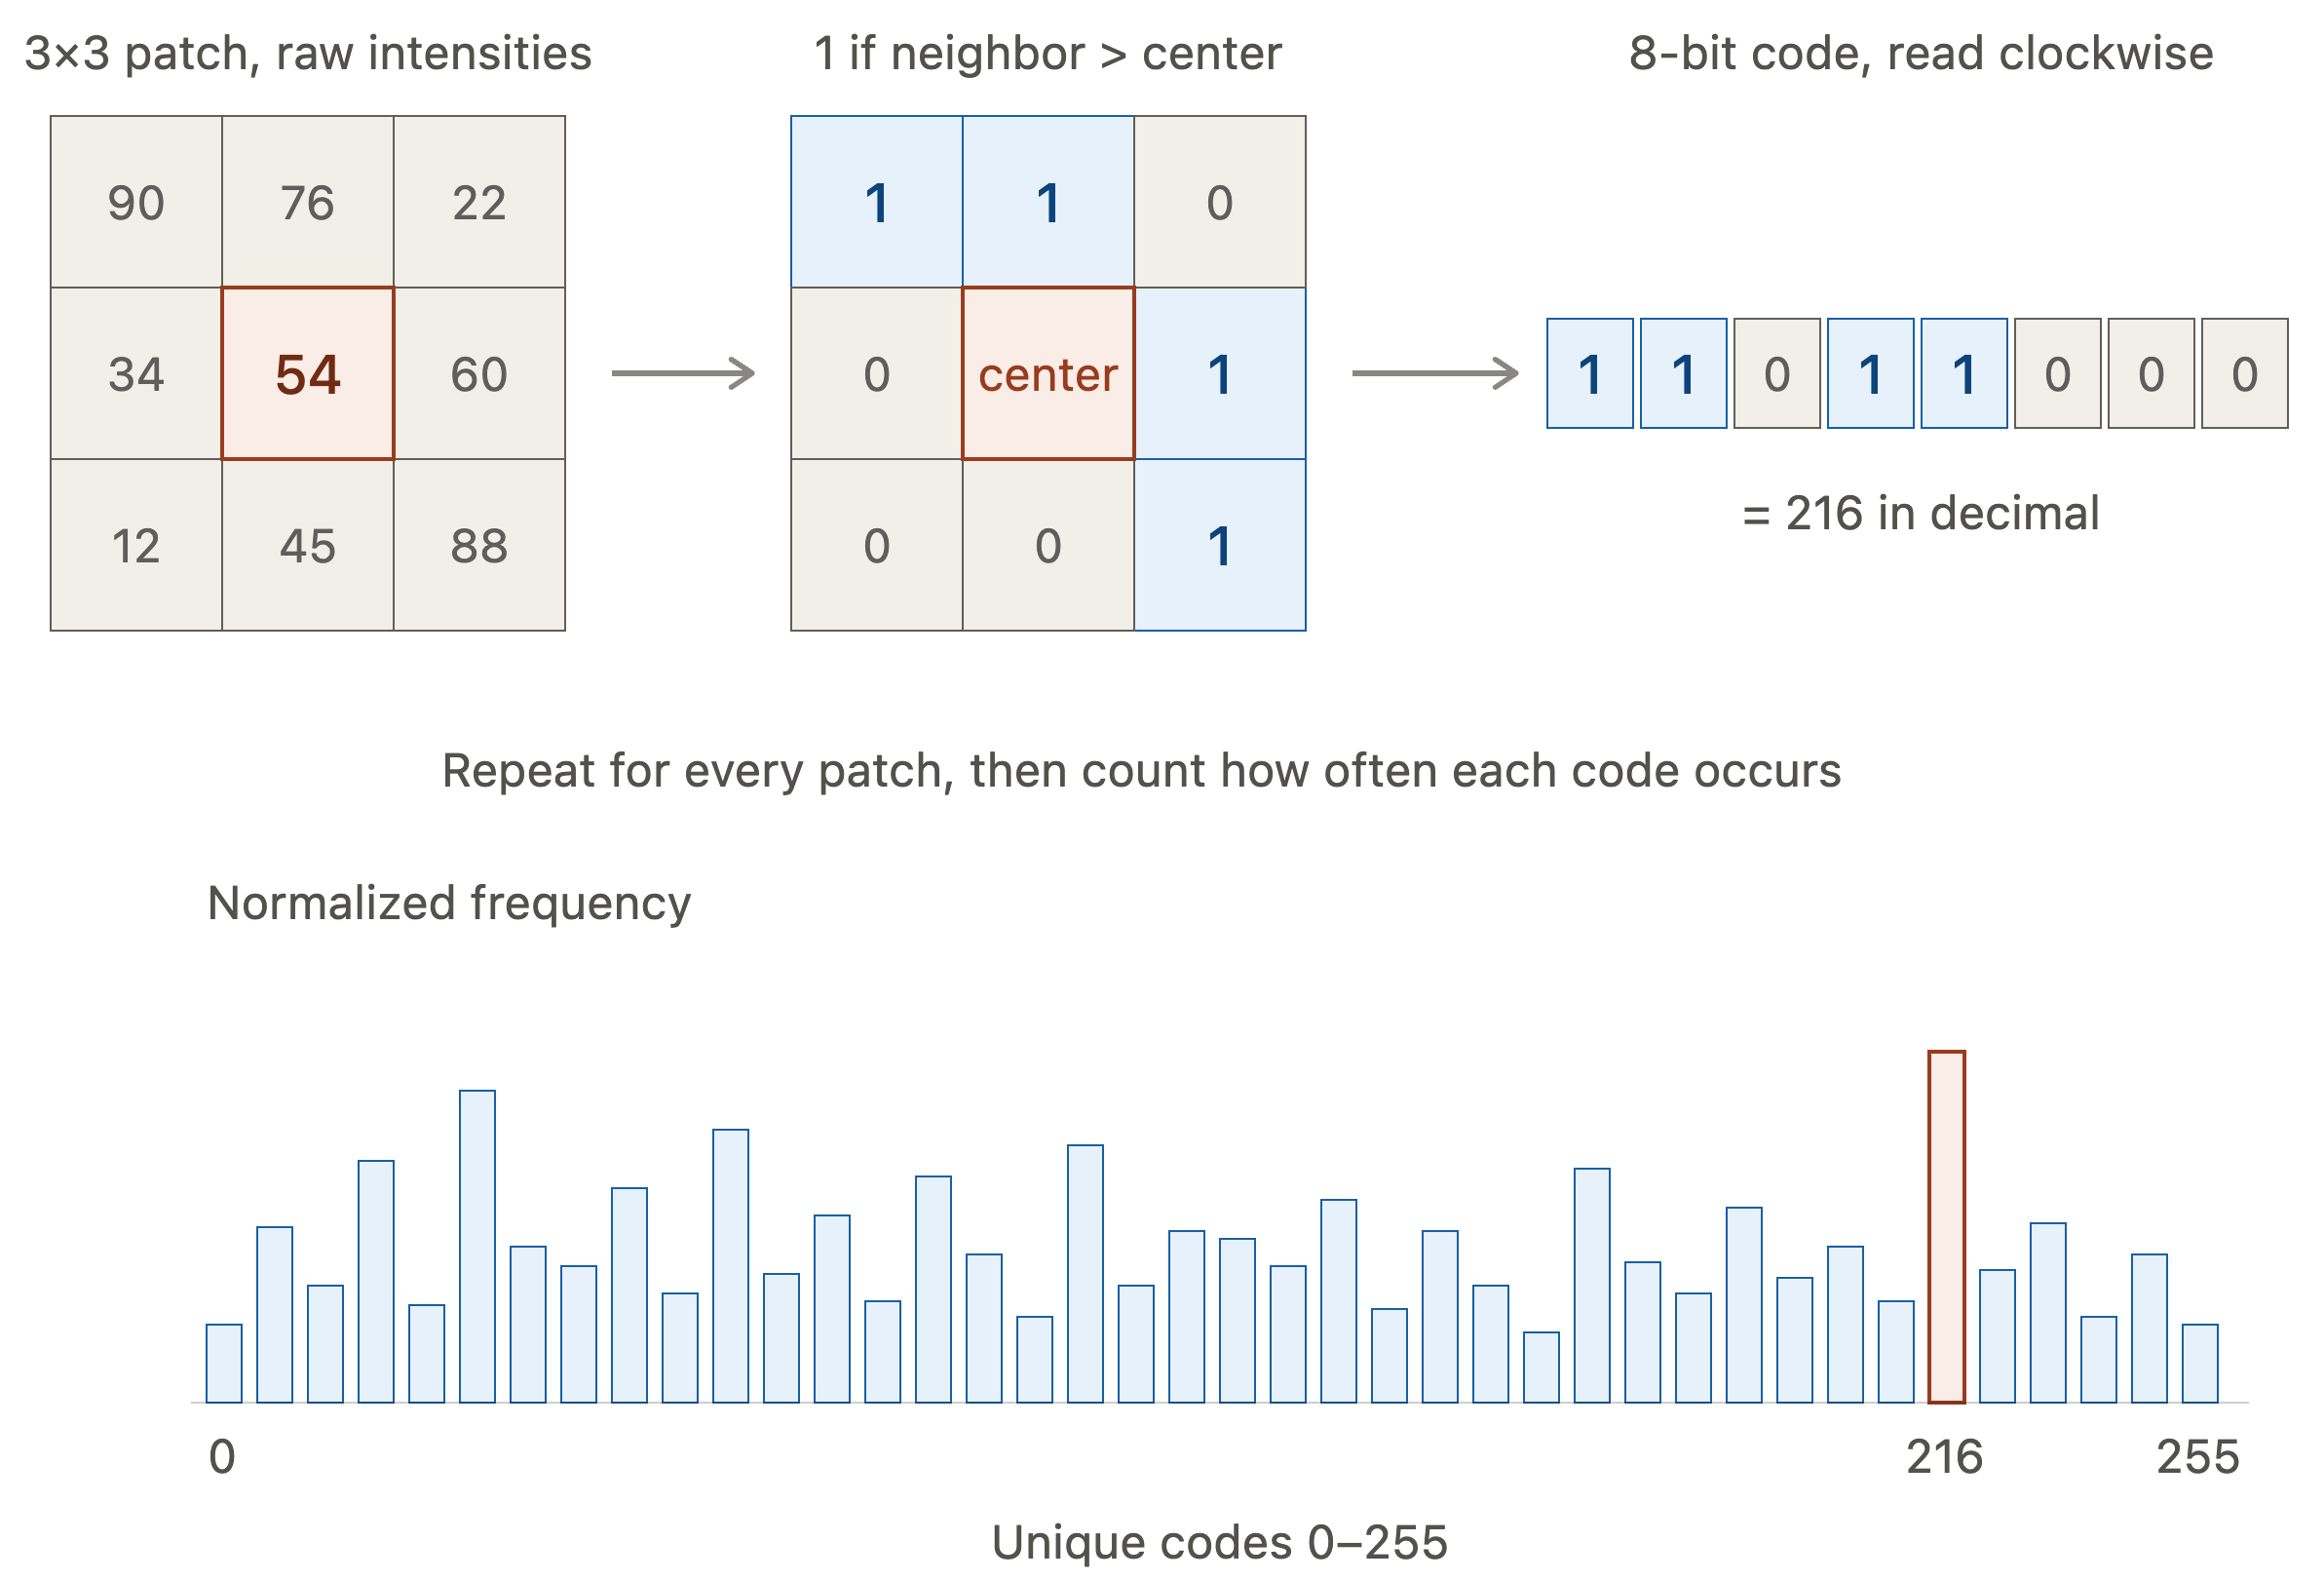
\includegraphics[scale=0.1]{lbp_computation.png}
\caption{Local Binary Pattern computation.} \label{lbp}
\vspace{-10pt}
\end{figure}

Local Binary Pattern (LBP) \cite{ojala2000gray} is a visual descriptor used for extracting and recognizing textures. It has been successfully applied to texture-based classification problems since then \cite{pietikainen2011computer,ke2013research,huang2011local}. LBP assigns a code to a fixed size pixel patch around a center pixel. For all possible patches in the image, a corresponding code of size n-1 is created, where n is the number of pixels in the patch.  For each pixel in the patch (excluding the center pixel), a 1 is recorded for the code if the intensity of the pixel is greater than the center pixel. A normalized histogram of number of patches versus unique codes can then be used as a fingerprint of the texture. The process is shown in Figure \ref{lbp}. This histogram can then be used as a feature and can be compared with a histogram generated from a test patch. One of several histogram comparison methods can then be used like Bhattacharyya (Hellinger) \cite{bhattacharyya1943measure,hellinger1909neue}, Chi-squared \cite{pearson1900criterion}, KL-Divergence \cite{kullback1951information} or Jensen-Shannon \cite{lin1991divergence}. Local Ternary Pattern (LTP) is an enhancement proposed to LBP to capture contrast, encoding higher or lower pixel intensity as a +1, 0, -1 ternary feature vector \cite{tan2007enhanced}. Alternatively, a split (Completed) LTP \cite{rassem2014completed} keeps the codes binary by splitting the codes into high (+1) and low (-1) codes. In this paper, we use the split-LTP variant. Aside from being easier to work with, it maps to biologically plausible center-surround receptive fields \cite{kuffler1953discharge}, with the high code being off-center on-surround and the low code being on-center off-surround. Split LTP therefore can behave similarly to center-surround receptive fields. 
In our preliminary testing, we saw that LTP was more robust to the choice of tolerance than LBP, and the observed performance metrics were higher than those of LBP. In addition, LTP has a stronger biological inspiration, as mentioned above. Therefore, we used LTP for all further experiments.

These feature descriptors are well suited for a sensorimotor system like Monty, unlike deep-learning-based learned features, as they do not need a pre-training step and do not suffer from training distribution limitations. Such low-level feature descriptors map well to ‘low-level’ feature detectors in the visual pathway. Another popular feature detector could be Gabor filters \cite{gabor1946theory}, which have been used for texture detection \cite{grigorescu2002comparison,arivazhagan2006texture}. As compared to LTP, Gabor filters have higher comptue cost because it requires running heavy 2D convolutions per patch. LTP's binary comparisons are much cheaper. Therefore, we use split LTP features for their robustness to the choice of tolerance, speed of computation and as a biologically inspired mechanism. The LTP feature (a histogram of the patch) is extracted in the sensory module of Monty and stored in the graph with other features like color as Hue-Saturation-Value (HSV).  

\section{Methods}

\subsection{Problem}

Monty has shown promise in identifying objects in the YCB dataset, but currently it is unable to distinguish objects with the same shape but different surface textures. It employs a simple hue-based feature detector to differentiate objects with similar shape. We need to test that adding the LTP non-morphological features helps in distinguishing objects of similar shape but different surface textures. In this section we describe the selection of datasets, baselines and test scenarios, including metrics used for the experiments and the experimental protocol.  


\subsection{Datasets}
\begin{figure}[!ht]
\centering
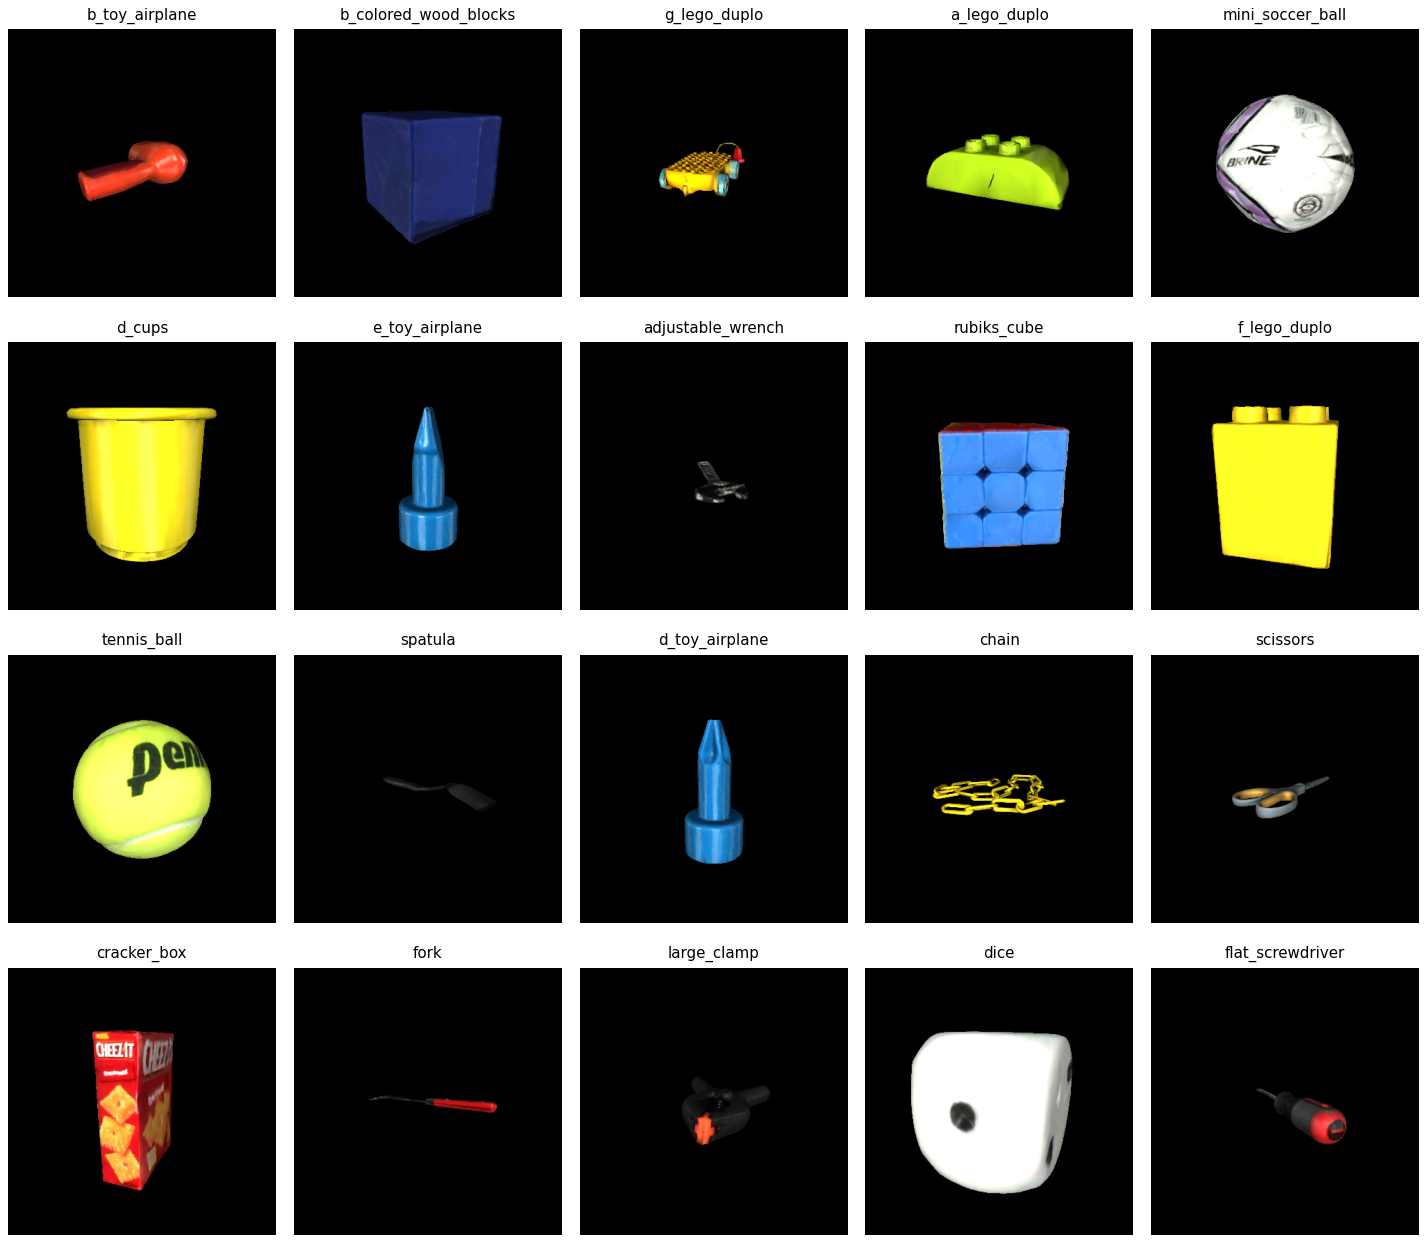
\includegraphics[scale=0.3]{ycb77_objects.png}
\caption{A subset of objects in the YCB dataset \cite{calli2015ycb}.} \label{ycb}
\end{figure}

Experiments were performed using the YCB object and model set \cite{calli2015ycb}. The dataset includes images and three-dimensional models of everyday household items used for benchmarking robotic manipulation, shown in Figure \ref{ycb}. The dataset provides various shapes, sizes, and textures, allowing for evaluation across a wide range of scenarios. Here we test Monty on 77 household items in the YCB dataset. The YCB dataset has been a standard benchmark used with Monty. 



\begin{figure}[!ht]
\centering
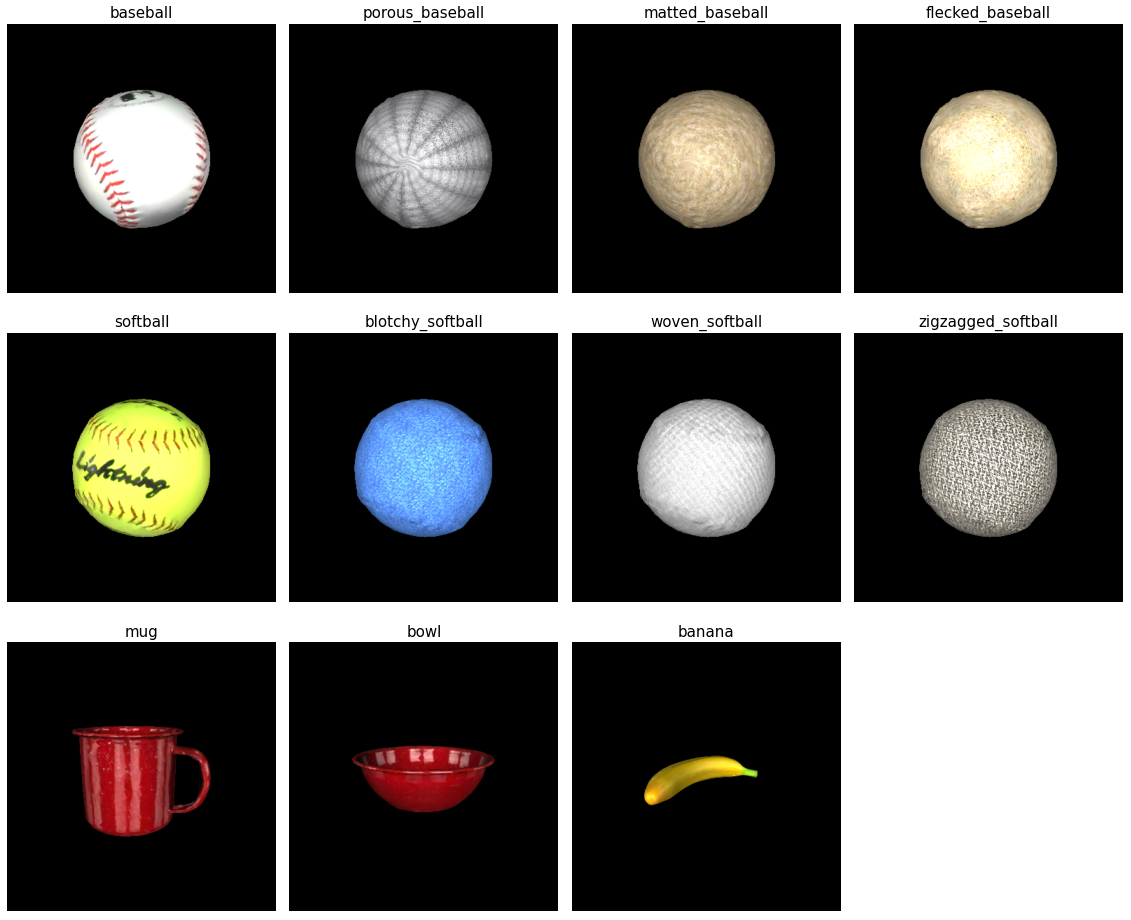
\includegraphics[scale=0.4]{retextured11_objects.png}
\caption{All objects in the YCB-11R dataset.} \label{YCB-11R}
\vspace{-.5cm}
\end{figure}
 
In addition, we create a specialized dataset for testing LTP features in extreme situations where the objects have the same shape but differ in texture models applied to them. For this, we exported the softball and baseball objects from YCB into Blender (TM) and re-textured them with 4 different textures each. We also added 3 different objects, which are banana, mug, and bowl, to prevent system regression and maintain generalization. This gave us a dataset of 11 objects, shown in Figure \ref{YCB-11R}. We created these variants by mixing similar hues and textures to increase the challenge. We used this dataset, called ‘YCB-11R’, to present a harder test case for LTP experimentation with Monty.  


% \begin{table}[!ht]
%     \caption{Mean and Std Dev of steps to convergence for the `4x4' environment.}
%     \vspace{.2cm}
%     \centering
%     \begin{tabular}{|c|c|c|c}
%     \hline
%     \textbf{Setting} & \textbf{Mean $\pm$ Std Dev} ($\downarrow$) & \textbf{\% Samples Converged}\\
%     \hline
%         Episodic Memory    & 211.69 $\pm$ 235.78 & 93\% \\
%         No Episodic Memory & 762.64 $\pm$ 287.76 & 52\% \\
%     \hline
%     \end{tabular}
%     \label{tab:results4x4}
% \end{table}



%\begin{table}[!ht]
%    \caption{Mean and Std Dev of steps to convergence}
%    \vspace{.2cm}
%    \centering
%    {\renewcommand{\arraystretch}{1.5}
%    \begin{tabular}{|c|c|c|c|c|}
%    \hline
%    & \multicolumn{2}{c|}{\textbf{4x4}} & \multicolumn{2}{c|}{\textbf{8x8}} \\
%    \hline
%    \textbf{Setting} & Mean $\pm$ Std Dev ($\downarrow$) & \% Converged & Mean $\pm$ Std Dev ($\downarrow$) & \% Converged\\
%    \hline
%        Episodic Memory    & 211.69 $\pm$ 235.78 & 93\% & 654.51 $\pm$ 361.85 & 53\% \\
%        No Episodic Memory & 762.64 $\pm$ 287.76 & 52\% & 971.05 $\pm$ 106.78 & 10\% \\
%    \hline
%    \end{tabular}
%    }
%    \label{tab:results}
%\end{table}



\subsection{Test conditions: Encoding schemes}

We use three different encoding strategies of LTP for comparison and testing, i.e. ‘ror’, ‘uniform’, and ‘multiscale’ \cite{ji2018MedianLocalTernary}. For LTP comparison, all possible code combinations are treated as unique unless a variant specifies otherwise, e.g.: a 3x3 grid will have 256 unique codes for 8 pixels surrounding the center pixel. Each one is described as follows: 

\begin{itemize}
    \item `ror': Codes are rotation invariant. Each code that can be rotated to one of the other codes is treated the same as the other. E.g.: (00000111, 00001110, 00011100, ...) are all put in the bin of 00000111. 

    \item 'uniform': A code is called uniform, or smooth, if it contains at most two transitions between 0 and 1 when the code is read circularly. For example, 00000000 and 00011100 are uniform (zero and two transitions), while 01010100 is not (six transitions). Each uniform code gets its own bin, and all non-uniform codes are collected into a single additional bin. For the 8 neighbors of a 3x3 patch, this reduces the histogram from 256 bins to 59, i.e. 58 uniform codes plus the catch-all bin. 

    \item `multiscale': The multiscale variant uses larger patch sizes. All computations remain the same and are done with the center pixel as the reference, leading to longer codes. Histograms from all patch sizes are concatenated. We use histograms with codes combined from radius 1, 2 and 3 for multiscale analysis.

\end{itemize}

\subsection{Experimental Protocol}\label{sec:protocol}

Experiments were constructed using the Monty agent\footnote{Code available at https://github.com/pulinagrawal/tbp.monty/tree/bica-exp} as the object recognition system. As typical with Monty, the objects are instantiated in the Habitat environment \cite{habitat19iccv} along with the agent sensor, as shown in Figure \ref{patch}. The baseline implementation was modified to include LTP in the object recognition pipeline.  

\begin{figure}[!ht]
\centering
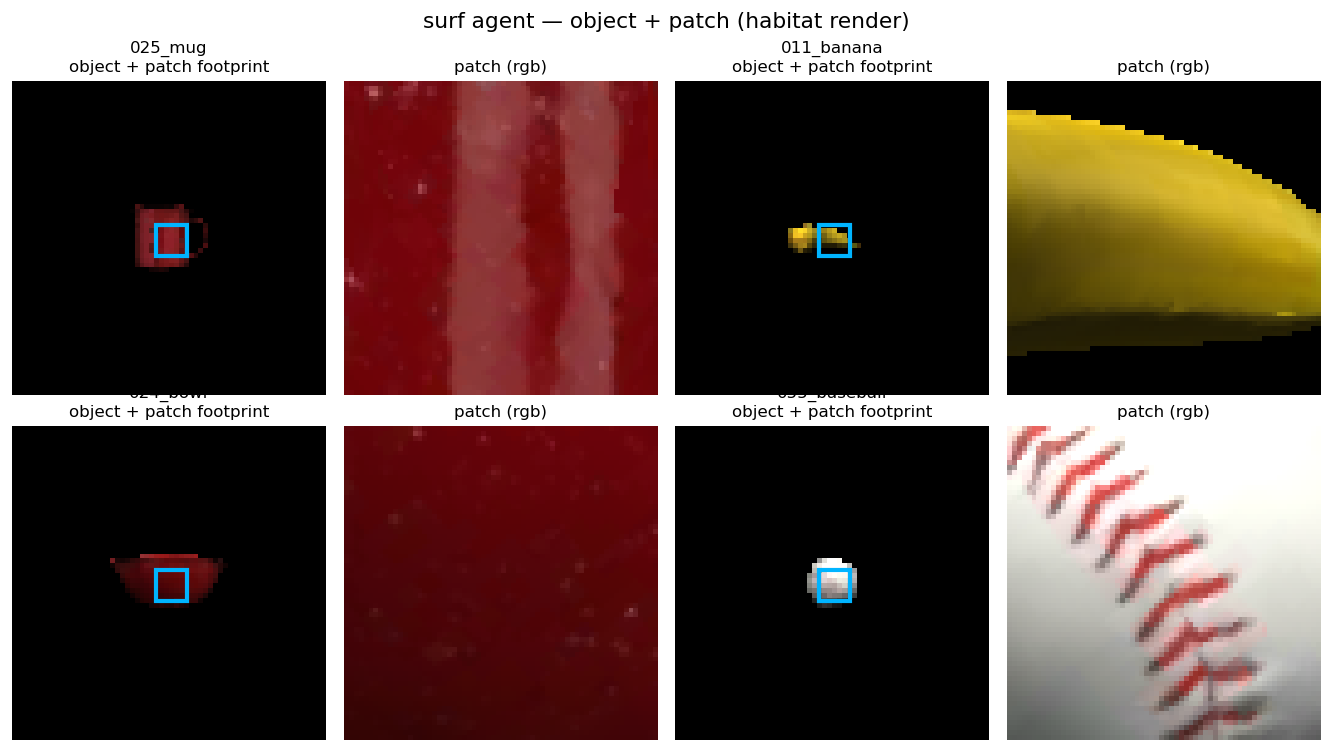
\includegraphics[scale=0.4]{object_patch_surf.png}
\caption{Sensor module patch visualization on various objects of the datasets.} \label{patch}
\end{figure} 

Training happens over 14 epochs, where one epoch runs an episode of training for an object from one of 14 possible viewpoints, i.e. from all 8 corners and 6 sides. In one episode, the sensor moves across the surface of the object at a constant distance away from it, using a predefined algorithmic policy and sensing a 64x64 patch. Figure \ref{patch} shows examples of patches from various objects. It records 1000 observations of various points on the surface of the object. This completes an episode for an object.  This graph of ‘features at pose’ thus collected is labeled with the object and given to the learning module. Over multiple epochs, if the same object is given to the learning module, it checks all the points already stored and prunes any suspected redundancies.

\begin{figure}[!ht]
\centering
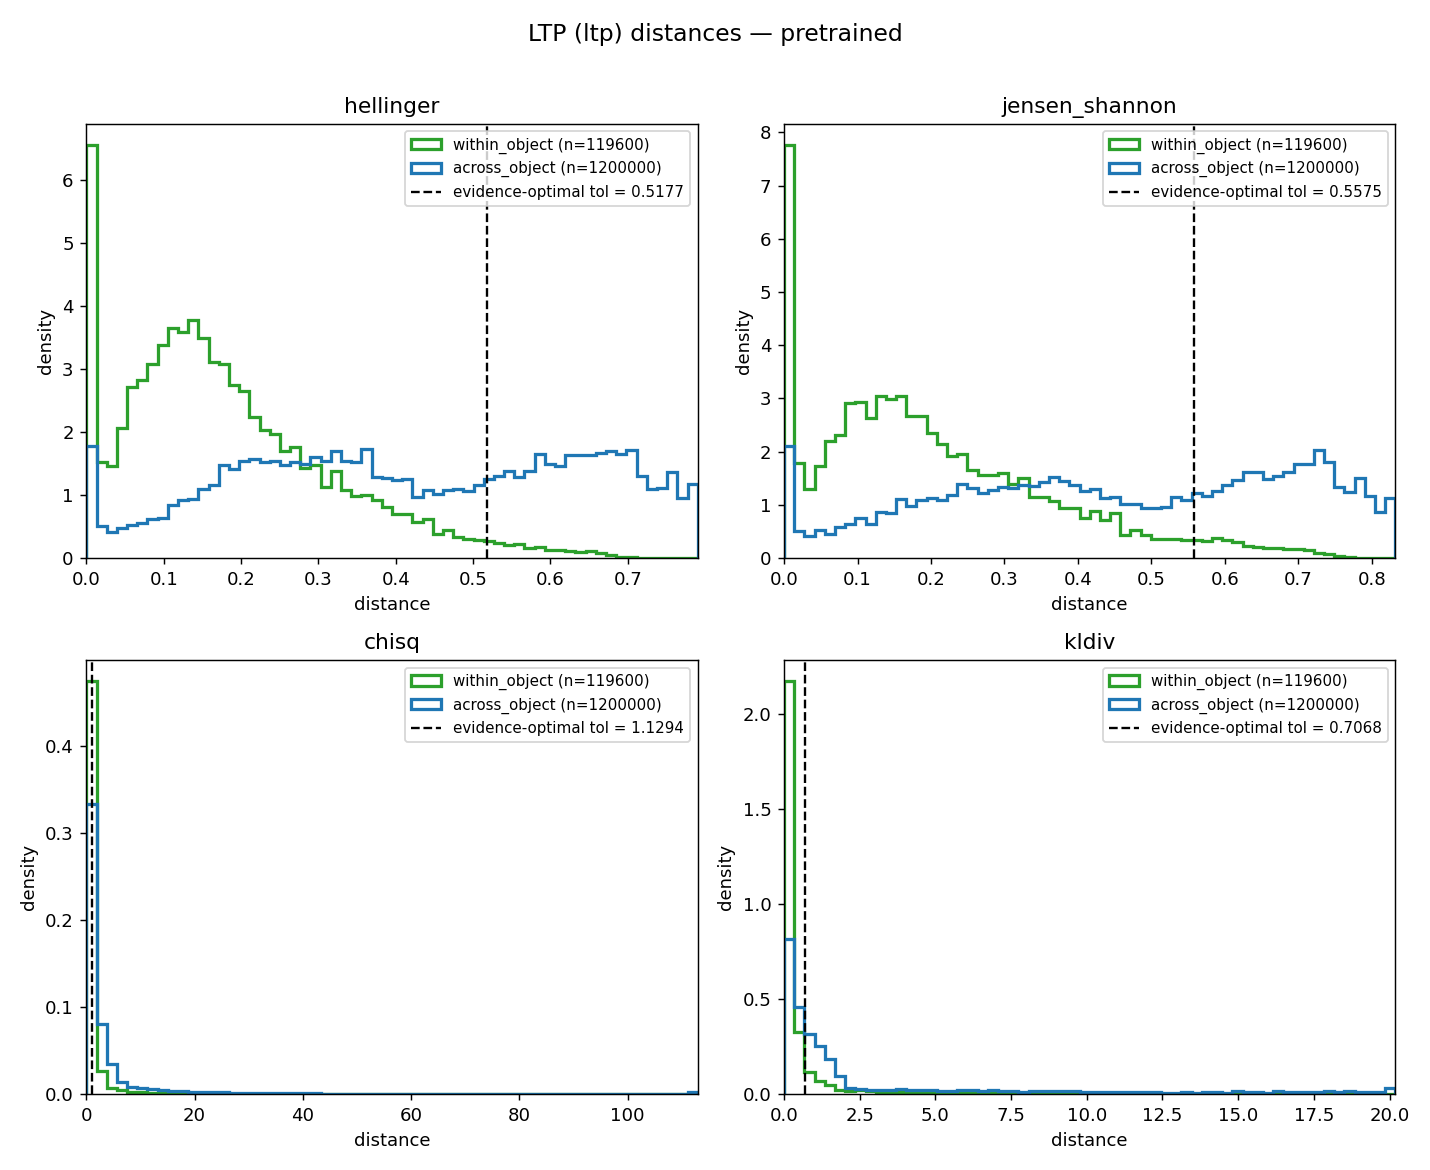
\includegraphics[scale=0.4]{surf_YCB-11R_ltp_distances_4metrics.png}
\caption{Plot showing the spread of distances between within object and across object patches on the `YCB-11R' dataset on training data.} \label{distances}
\vspace{-.75cm}
\end{figure}

For evaluation, all the pretrained graphs are loaded and frozen. We perform a simple threshold selection for setting the tolerance of the LTP feature that maximizes the difference in evidence collection for a patch under test on the same object versus a different object using the patch level graph data stored during training (no testing data is used for threshold selection). This analysis is done in tandem with the selection of an appropriate distance metric. This helps us develop a rigorous LTP histogram matching system that can be used by Monty for texture differentiation. A plot of patch distances on 'ror' encoded LTP with various distance metrics is shown in Figure \ref{distances}. Bhattacharyya (Hellinger) distance, being a normalized metric with high discriminative power due to its low spread of distances, was thus selected based on this analysis. The tolerance is determined by the value that maximizes the difference of mean evidence gathered within the object and between objects. The analysis indicates a tolerance value close to 0.5 is appropriate to achieve highest separation. 

A test sample is an object in a random rotation (excluding the training rotations). An epoch presents one test sample of each object in the dataset to Monty, one at a time. Monty uses a predefined algorithmic policy (different from the training policy) to pick a point to move next that could maximally discriminate the remaining hypotheses. Each move accumulates evidence for the hypotheses as described in Section 2.4. Once the maximum number of steps (500 is typical and used here for experiments) is reached, or there is only one hypothesis left, the system reports the recognition based on the hypothesis with the most evidence. Each object is presented in a new random rotation, excluding the training rotations, for a few epochs (10-20 epochs are typical in the Monty framework and used here for experiments). The recognition accuracy and average number of steps to convergence are reported as the final results.

We use HSV as the only non-morphological feature as the baseline for all experiments. The HSV non-morphological feature is extracted from the center pixel of sensed patch. We use this HSV feature setting enabled as the baseline because that is the current default in Monty.

\subsection{Evaluation Metrics}

We use `percent\_correct' $\uparrow$ (overall recognition accuracy) and `avg\_convergence\_steps' $\downarrow$ (average number of steps before convergence) as our primary evaluation metrics. In addition to accuracy, convergence rate becomes an important metric in the context of a sensorimotor system like Monty because it is not asked to recognize an object in a single presentation. Monty moves its sensor(s) over the object and only sees a small patch at a time. Therefore, fewer steps to convergence mean higher recognition speed. 
%In addition, we report some auxiliary metrics. First, the `percent\_use\_mlh' $\downarrow$ i.e. percentage of presentations where timeout happened due to maximum number of steps reached and most-likely-hypothesis was used for recognition. Second, `percent\_correct\_mlh' $\uparrow$ i.e. percentage of samples where the most-likely-hypothesis was used. We also test the system under various ablations of noise and rotation.  

\section{Results}
\begin{table}
    \vspace{-1cm}
    \setlength{\tabcolsep}{4pt}
    \renewcommand{\arraystretch}{1.25}
    \vspace{.1cm}
    \centering
    \begin{tabular}{l|l|r|r}
    \hline
    \textbf{HSV} & \textbf{LTP} & \textbf{percent\_correct ($\uparrow$)} & \textbf{avg\_convergence\_steps($\downarrow$) $\pm$ SEM}\\
    \hline \hline
             \cross & \cross     & 46.82 & 366.63 $\pm$ 14.39\\\hline
             \cross & ror        & 78.18 & 354.79 $\pm$ 14.68\\\hline
    \baserow \tickm & \cross     & 93.18 & 218.69 $\pm$ 15.24\\\hline
             \tickm & uniform    & 96.81 & 183.52 $\pm$ 14.74 \\\hline
             \tickm & multiscale & 95.90 & 181.06 $\pm$ 14.68\\\hline
             \tickm & ror        & 96.81 & 185.45 $\pm$ 14.73\\\hline

    %\cross & ror    & 65.45 & 366.50 \\
    \end{tabular}
    \vspace{.1cm}
    \caption{LTP performance on the YCB-11R dataset in ambient lighting. The shaded row is the baseline (Monty default: HSV only); rows below it are the LTP test conditions.}
    \label{tab:11retexture_amb}
    \vspace{-1cm}
\end{table}
To test the applicability of using LTP features to recognize objects we tested the recognition accuracy (as `percent\_correct') and steps to convergence (as `avg\_convergence\_steps') on the YCB dataset and a custom YCB-11R dataset. We presented each of the 11 objects in the dataset with 10 random rotations to Monty for a total of 110 test samples for the directional lighting and with 20 random rotations for a total of 220 samples for the ambient lighting setups, equally divided between the objects. For the larger YCB dataset, we tested each of the 77 objects with 3 random rotations each for a total of 231 test samples.

Results for the YCB-11R dataset with various LTP encoding schemes under ambient lighting conditions are shown in Table \ref{tab:11retexture_amb}. We compare the various LTP encoding schemes on the more challenging directional lighting setup with YCB-11R dataset, see Table \ref{tab:11retexture}. We tested YCB-11R dataset with both ambient (Table \ref{tab:11retexture_amb}) and directional (Table \ref{tab:11retexture}) lighting setup to understand its generalization capability.  

\begin{table}
    \vspace{-.5cm}
    \setlength{\tabcolsep}{4pt}
    \renewcommand{\arraystretch}{1.25}
    \vspace{.1cm}
    \centering
    \begin{tabular}{l|l|r|r}
    \hline
    \textbf{HSV} & \textbf{LTP} & \textbf{percent\_correct ($\uparrow$)} & \textbf{avg\_convergence\_steps ($\downarrow$) $\pm$ SEM} \\
    \hline \hline
             \cross & \cross     & 45.45 & 370.87 $\pm$ 20.20\\\hline
             \cross & ror        & 65.45 & 366.50 $\pm$ 20.42\\\hline
    \baserow \tickm & \cross     & 89.09 & 275.82 $\pm$ 22.19\\\hline
             \tickm & uniform    & 90.00 & 280.36 $\pm$ 22.00\\\hline
             \tickm & multiscale & 91.81 & 243.75 $\pm$ 21.84\\\hline
             \tickm & ror        & 94.54 & 243.96 $\pm$ 21.89\\\hline

    %\cross & ror    & 65.45 & 366.50 \\
    \end{tabular}
    \vspace{.1cm}
    \caption{LTP performance on the YCB-11R dataset in directional lighting. The shaded row is the baseline (Monty default: HSV only); rows below it are the LTP test conditions.}
    \label{tab:11retexture}
    \vspace{-1cm}
\end{table}
Since `ror' performed the best among the three encoding schemes, we tested that on the larger YCB dataset. We can see from Table \ref{tab:77obj} that for the YCB dataset the accuracy was close to 100\% even without any non-morphological features. This is due to the fact that the shape of the objects in YCB dataset are very discriminating. But using HSV, the accuracy is pushed up to 100\%. With HSV and `ror' LTP combined the average number of steps for convergence goes down further. 
\begin{table}
    \setlength{\tabcolsep}{4pt}
    \vspace{-.5cm}
    \renewcommand{\arraystretch}{1.25}
    \vspace{.1cm}
    \centering
    \begin{tabular}{l|l|r|r}
    \hline
    \textbf{HSV} & \textbf{LTP} & \textbf{percent\_correct ($\uparrow$)} & \textbf{avg\_convergence\_steps ($\downarrow$) $\pm$ SEM} \\
    \hline \hline
    %\cross & \cross & 45.45 & 371.53 \\\hline
             \cross & \cross & 99.56 & 96.45 $\pm$ 9.90 \\\hline
    \baserow \tickm & \cross & 100   & 53.12 $\pm$ 6.50 \\\hline
             \tickm & ror    & 100   & 49.64 $\pm$ 5.80 \\\hline
    %\cross & ror    & 65.45 & 366.50 \\
    \end{tabular}
    \vspace{.1cm}
    \caption{LTP performance on the YCB dataset in directional lighting. The shaded row is the baseline (Monty default: HSV only).}
    \label{tab:77obj}
\end{table}
\vspace{-1.5cm}
\section{Discussion}

Our experimental results demonstrate that LTP is a strong addition to Monty to improve its object recognition capability, especially using the 'ror' encoding scheme. It significantly increases the speed of object detection as measured by the `avg\_convergence\_steps' while boosting the overall accuracy of detection. We evaluated the accuracy improvements using the exact McNemar's test, and the convergence spped was evaluated using the Wilcoxon signed-rank test. We could use the paired versions of the tests because the same objects were tested with the same random seeds which tested them at same angles. We observed the improvements in accuracy and convergence speed were significant with p = 0.0078 and p < 0.0001 for the respective tests. Our YCB-11R dataset presented a challenge to Monty beyond what the YCB dataset can typically provide. On YCB morphology alone, without color, is sufficient for almost complete separation. LTP was able to show an improvement in accuracy with the YCB-11R dataset in addition to reduced convergence rate. We observe that HSV features substantially improves the accuracy over the baseline without any non-morphological features. But upon using any form of LTP the accuracy improves further and the average number of steps needed to recognize an object reduces. Furthermore, consistent benefit is observed with LTP even under directional lighting. Directional lighting is possibly a harder challenge than realistic room lighting conditions in Habitat because directional lighting in Habitat leaves the unlit area extremely dark. With this improved capability, Monty can distinguish objects with similar color profiles by using differences in surface texture patterns.  

\section{Conclusion}
This work demonstrates that the integration of Local Ternary Patterns (LTP) into the Monty sensorimotor system improves object recognition in scenarios where shape alone is insufficient. By adjusting Monty’s existing feature extraction methods by adding texture descriptors, the system gained a non- morphological feature that can help distinguish objects that have similar geometric shapes but different surface characteristics. We note that we do not compare this to other SOTA benchmarks because Monty is a biologically-inspired system, whose approach to embodied learning is substantially different from the current deep learning methodologies. The work here will help develop this neocortex-inspired system to develop further and any advancements to this system will ultimately help inform the development of embodied sensorimotor agents. 

While these initial results show that implementing LTP improves object recognition, there are still areas for future work. First, we will undertake the task of testing the system under different background conditions and different datasets to validate the general applicability of the method. Secondly, we plan on testing this setup with an actual robotic arm to test the method’s applicability in the real world to rapidly recognize objects and understand their morphology without the need for retraining the visual system. Finally, we plan on transitioning the texture histograms created by LTP into Hierarchical Temporal Memory (HTM) \cite{hawkins_hierarchical_2011} Spatial Pooler based texture representations. This will ultimately align the pipeline to the core principles from Numenta out of which the Thousand Brains Theory was established.   

\begin{credits}
\subsubsection{\ackname} Part of the work done for this study came from a Senior Design Project sponsored by Thousand Brains Project at Penn State Behrend's School of Engineering. We would like to thank Ryan Adeli, Anthony Velcko, Tristan Somlinski and Niels Leadholm for their contributions and guidance which made this work possible.

\subsubsection{\discintname}
The authors have no competing interests. 
\end{credits}

\bibliographystyle{splncs04}
\bibliography{ExportedItems}
%\bibliography{htm-rl}
\end{document}